\section{Code Design}
\label{Sect:CodeDesign}

\subsection{General Code Structure}

The main body of the tracker code is implemented as three distinct MAUS map modules and, at present, one reducer module.  There also exist various helpful top-level user tools, and the tracker geometry, calibration and configuration files. A diagram showing the tracker software data flow with the corresponding modules is shown in figure~\ref{Fig:DataFlow}, with the following sections expanding on each area.

\begin{figure}[p]
  \begin{center}
    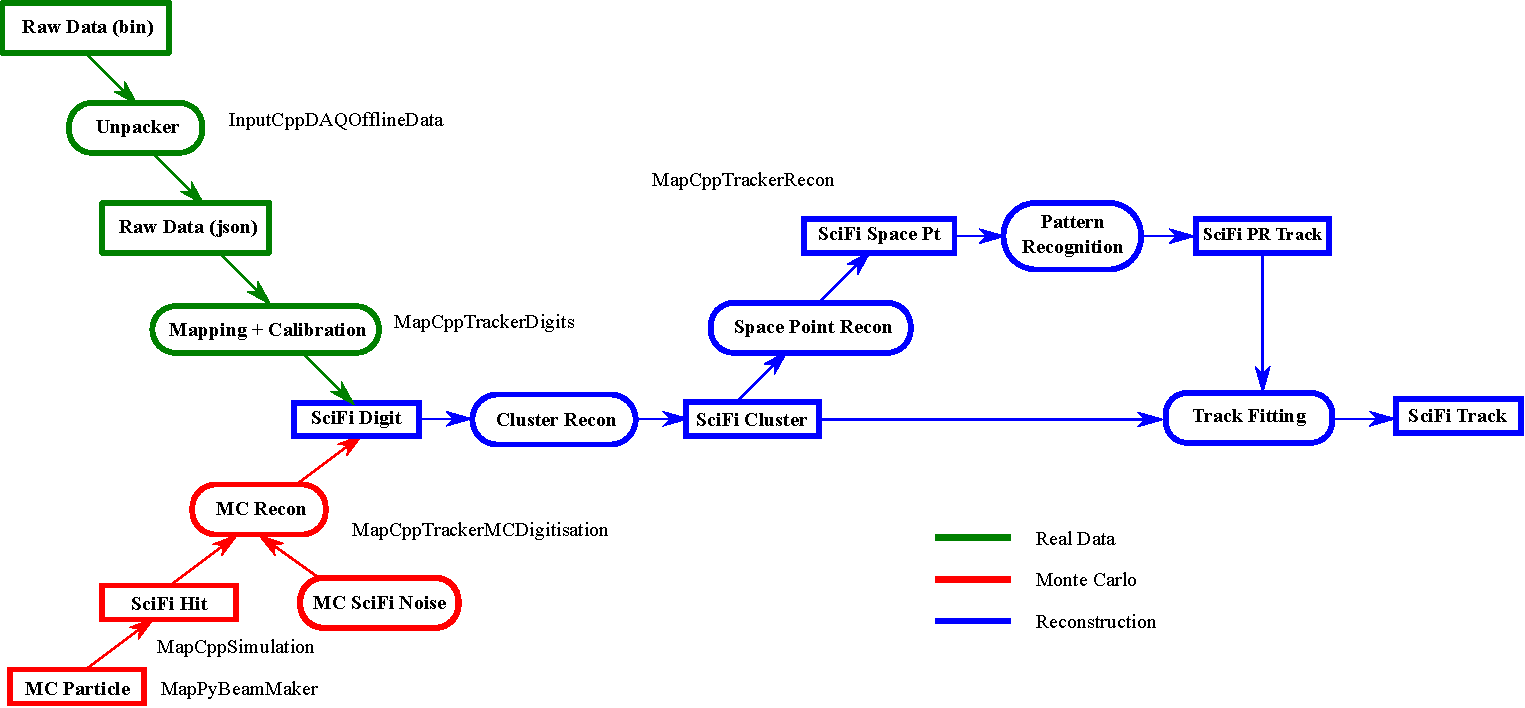
\includegraphics[width=1.10\textwidth, angle=90]{detectors/tracker/06-CodeDesign/Figures/DataFlow.pdf}
  \end{center}
  \caption{Schematic of the tracker software data showing MC and Real data input, and subsequent reconstruction. MAUS modules corresponding to given process are indicated (MapCppTrackerRecon encompasses all of the reconstruction, shown in blue).  Once digits have been formed, reconstruction is agnostic as to whether the MC or Real path was followed.}
  \label{Fig:DataFlow}
\end{figure}

\subsubsection{MapCppTrackerDigits}
This map is used to digitise real data.  It calls on additional functionality from the RealDataDigitisation class, which is stored in \verb;src/common_cpp/Recon/SciFi;.

\subsubsection{MapCppTrackerMCDigitisation}
This map is used to digitise Monte Carlo data.

\subsubsection{MapCppTrackerRecon}
This map performs the main reconstruction work, moving from digits to cluster to spacepoints to pattern recognition tracks, and finally full Kalman tracks. Most work is farmed out to backend C++ classes. The following are the top level classes for each stage of the reconstruction, and are stored in \verb;src/common_cpp/Recon/SciFi;:

\begin{itemize}
 \item SciFiClusterRecon - cluster reconstruction from digits
 \item SciFiSpacepointRecon - spacepoint reconstruction from cluster
 \item PatternRecognition - association of spacepoints to tracks, and crude initial track fit
\end{itemize}
The backend classes for the final track fit are stored under \verb;src/common_cpp/Recon/Kalman; and  \verb;src/common_cpp/Recon/Bayes;, the top level class being KalmanTrackFit. Other classes used include:

\begin{itemize}
 \item KalmanFilter
 \item KalmanHelicalPropagator
 \item KalmanStraightPropagator
 \item KalmanState
 \item KalmanSeed
\end{itemize}

\subsubsection{ReduceCppPatternRecognition}
This reducer displays spacepoints and pattern recognition tracks by tracker, in the $x-y$, $x-z$ and $y-z$ projections, an example being shown in figure~\ref{Fig:SciFiReducerXYZ}.  It also creates an InfoBox, which displays various information for the spill and run, such as the number of clusters, spacepoints, etc.  The plots are made using ROOT TGraphs, and the InfoBox with a TPaveText. 

\begin{figure}[htb]
  \begin{center}
    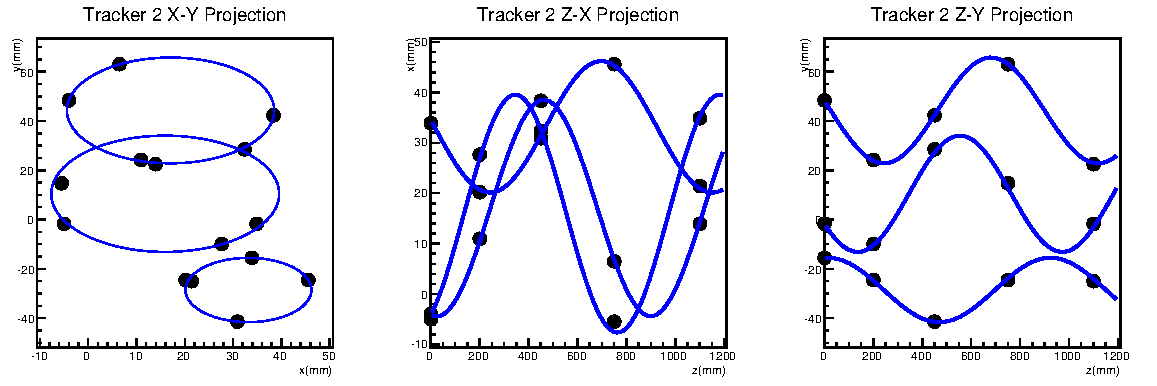
\includegraphics[width=0.8\textwidth]{detectors/tracker/06-CodeDesign/Figures/xyzPlotterOutput.pdf}
  \end{center}
  \caption{Output from the pattern recognition reducer showing the real space projections of a three event spill in tracker 2.}
  \label{Fig:SciFiReducerXYZ}
\end{figure}

\subsubsection{Reducer Backend}

The backend classes for the reducers are held in \verb;src/common_cpp/Plotting/SciFi;.  They consist of a reduced tracker data container class, TrackerData, a series of plotting class based on ROOT, and a manager class TrackerDataManager, used to populate the TrackerData and call the various plotters. The plotters themselves inherit from a base class, TrackerDataPlotterBase.  Each daughter class overloads the bracket operator, taking in arguments of two TrackerData objects, one per tracker, and a ROOT TCanvas, to plot on.  The current types available are:

\begin{itemize}
 \item \textbf{Info Box}: displays various information on the spill and run in text
 \item \textbf{Spacepoints}: displays spacepoint positions in $x-y$, $x-z$, and $y-z$
 \item \textbf{Tracks}: displays pattern recognition tracks in $x-y$, $x-z$, and $y-z$ 
 \item \textbf{XYZ}: calls Tracks and Spacepoints to display them both together
  \item \textbf{SZ}: displays pattern recognition tracks in $s-z$ ($s$ being the distance swept out by a particle in the $x-y$ plane)
\end{itemize}

\subsection{Tracker configuration variables}

\renewcommand{\arraystretch}{1.0}
\begin{tabular}{| l | l | p{8cm} |}
  \hline                       
  \textbf{Variable} & \textbf{Default}& \textbf{Description}  \\
  \hline
  SciFiMUXNum & 7 & \\
  SciFiFiberDecayConst & 2.7 & \\
  SciFiFiberConvFactor & 3047.1 & \\
  SciFiFiberTrappingEff & 0.056 & \\
  SciFiFiberMirrorEff & 0.6 & \\
  SciFiFiberTransmissionEff & 0.8 & \\
  SciFiMUXTransmissionEff & 1.0 & \\
  SciFivlpcQE & 0.8 & \\
  SciFivlpcEnergyRes & 4.0 & VLPC energy resolution (MeV) \\
  SciFivlpcTimeRes & 0.2 & VLPC time resolution (ns) \\
  SciFiadcFactor & 6.0 & \\
  SciFitdcBits & 16 & \\
  SciFitdcFactor & 1.0 & \\
  SciFinPlanes & 3 & \\
  SciFinStations & 5 & \\
  SciFinTrackers & 2 & \\
  SciFiNPECut & 2.0 & \\
  SciFiClustExcept & 100 & \\
  SciFi\_sigma\_tracker0\_station5 & 0.4298 & Tracker 1 station 5 resolution (mm) \\
  SciFi\_sigma\_triplet & 0.3844 & Spacepoint triplet resolution (mm) \\
  SciFi\_sigma\_z & 0.081 & (mm) \\
  SciFi\_sigma\_duplet & 0.6197 & (mm) \\
  SciFiPRHelicalOn & True & Helical pattern recognition flag \\
  SciFiPRStraightOn  & True & Straight pattern recognition flag \\
  SciFiRadiusResCut & 150.0 & Helix radius cut (mm) \\
  SciFiNTurnsCut & 0.75 & Cut checking turns between stations is correct \\
  SciFiMaxPt & 180.0 & Transverse momn. upper limit cut used in pat rec \\
  SciFiMinPz & 180.0 & Longitudinal momn. lower limit cut used in pat rec \\
  SciFiPerChanFlag & 0 & \\
  SciFiNoiseFlag & 1.5 & \\
  SciFiCrossTalkSigma & 50.0 & \\
  SciFiCrossTalkAmplitude & 1.5 & \\
  SciFiDarkCountProababilty & 0.017 & Probability of dark count due to thermal electrons \\
  SciFiChannelCalibList & & Channel calibration data location \\
  SciFiParams\_Z & 5.61291 & \\
  SciFiParams\_Plane\_Width & 0.6523 & \\
  SciFiParams\_Radiation\_Legth & 424.0 & \\
  SciFiParams\_Density & 1.06 & \\
  SciFiParams\_Mean\_Excitation\_Energy & 68.7 & \\
  SciFiParams\_A & 104.15 & \\
  SciFiParams\_Pitch & 1.4945 & \\
  SciFiParams\_Station\_Radius & 160. & \\
  SciFiParams\_RMS & 370. & \\
  SciFiSeedCovariance & 1000 & Error estimate for seed values of the Kalman fit \\
  SciFiKalman\_use\_MCS & True & Flag to add multiple scattering to the Kalman fit \\
  SciFiKalman\_use\_Eloss & True & Flag to add energy loss to the Kalman fit \\
  SciFiUpdateMisalignments & False & Do a misalignment search and update \\
  SciFiKalmanVerbose & False & Dump information per fitted track \\
  \hline  
\end{tabular}
\renewcommand{\arraystretch}{1.0}



